\section{Theorie}
\label{sec:theorie}

Vorweg sei gesagt, dass die folgenden Überlegungen zum hier
durchgeführten Versuch aufgrund der Wechselwirkungen
zwischen Elektronen und Luftmolekülen
nur im Hochvakuum möglich sind.


\subsection{Austrittsarbeit und Energieverteilung}

Die hohe Leitfähigkeit von Metallen rührt aus ihrer kristallinen
Festkörperstruktur, in der praktisch alle Atome ionisiert sind.
So bildet sich ein periodisches Gitter, auf dem sich Elektronen 
als Leitungselektronen 'frei' bewegen können. \\

Das dabei vorherrschende Gitterpotential unterscheidet sich um
den Betrag $\Phi$ vom Außenraum und kann dabei näherungsweise
als konstant angenommen werden. \\

Möchte ein Elektron nun das Metall verlassen, muss es, wie in
\autoref{fig:abb1} dargestellt, den Potentialtopf verlassen,
sprich die Austrittsarbeit $\text{e}_0 \xi$ leisten. \\

\begin{figure}[H]
    \centering
    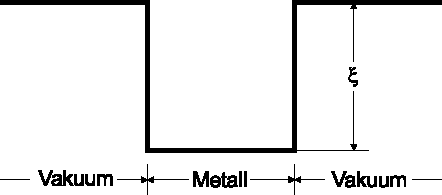
\includegraphics{figures/Abb1.pdf}
    \caption{Potentialtopfmodell eines Metalls\cite{ap09}.}
    \label{fig:abb1}
\end{figure}

Die Elektronen unterliegen dabei als Teilchen mit halbzahligem
Spin dem Pauli-Prinzip, das besagt, dass jeder mögliche
Zustand der Energie $E$ von höchstens zwei Elektronen mit
entgegengesetztem Spin eingenommen werden kann.
So besitzen Elektronen auch im absoluten Nullpunkt noch eine Restenergie,
die Fermische Grenzenergie $\zeta$. \\
Diese Grenzenergie ist bei Raumtemperatur $>> \text{k}_\text{B} T$. \\

Die Fermi-Diracsche Verteilungsfunktion beschreibt dabei die Wahrscheinlichkeit,
einen möglichen Zustand der Energie $E$ als besetzt vorzufinden. \\
Sie besitzt die Form
\begin{equation}
    f(E) = \dfrac{1}{\text{exp}(\frac{E - \zeta}{\text{k}_\text{B} T} + 1)} \,,
\end{equation}
ihr Verlauf ist in \autoref{fig:abb2} dargestellt.

\begin{figure}
    \centering
    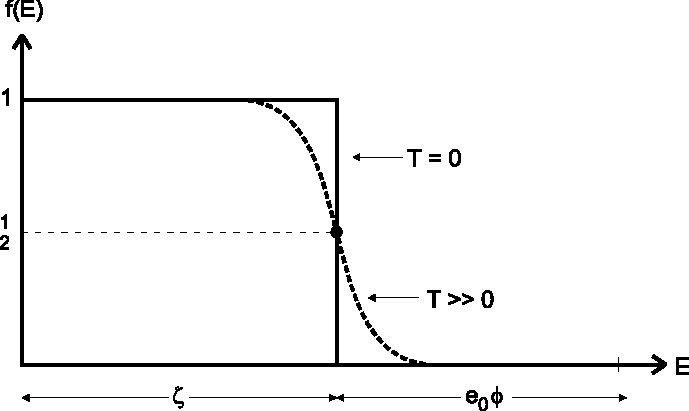
\includegraphics{figures/Abb2.pdf}
    \caption{Verlauf der Fermi-Diracschen Verteilungsfunktion am absoluten Nullpunkt \cite{ap09}.}
    \label{fig:abb2}
\end{figure}

Die dabei zum Verlassen des Metalls nötige Energie $\zeta + \text{e}_0 \Phi$
ist